\documentclass{article}

\usepackage{listings}
\usepackage{url}
\usepackage{hyperref}
\usepackage{graphicx}
\usepackage{xepersian}
\usepackage{ulem}


\settextfont{XB Zar}
\setlatintextfont{XB Zar}


\makeatletter
\let\@@scshape=\scshape
\renewcommand{\scshape}{%
  \ifnum\strcmp{\f@series}{bx}=\z@
    \usefont{T1}{cmr}{bx}{sc}%
  \else
    \ifnum\strcmp{\f@shape}{it}=\z@
      \fontshape{scsl}\selectfont
    \else
      \@@scshape
    \fi
  \fi}
\makeatother

\title{
مستند فاز سوم پروژه
\\
\vspace{4mm}
سیستم‌های عامل
\\
\vspace{2mm}
دکتر جلیلی
}

\author{
محمدحسین اعلمی
\hspace{1cm}
۹۴۱۰۴۴۰۱
\\
محمدمهدی فاریابی
\hspace{1cm}
۹۳۱۰۱۹۵۱
}

\date{}
\begin{document}

\maketitle

\section*{مقدمه}

این مستند گزارش انجام فاز سوم پروژه درس سیستم‌های عامل به منظور آشنایی با زمان‌بندی پردازه‌ها، مدیریت حافظه و پیاده‌سازی یک شل نمونه است. تمامی عملیات‌های ذکر‌شده در مستند روی سیستم‌عامل
\lr{Ubuntu 16.04}
پیاده و تست‌ شده‌اند.

\section{گام اول - زمان‌بندی پردازه}

\subsection{بخش اول}

در بخش اول گام اول این فاز اطلاعات مربوط به برش‌های زمانی زمان‌بند هسته را استخراج می‌کنیم. در ابتدا توضیحاتی درباره نحوه زمان‌بندی پردازه‌ها در سیستم عامل لینوکس می‌دهیم.

\subsubsection{زمان‌بندی در هسته لینوکس\cite{1}\cite{2}}

در سیستم عامل لینکوس نحوه زمان‌بندی پردازه‌ها در طی تاریخ دچار تحولات زیادی شده است. شیوه زمان‌بندی که در حال حاضر روی هسته لینوکس استفاده می‌شود ترکیبی از شیوه‌های زمان‌بندی مختلف برای پردازه‌های مختلف است، به این معنی که همه‌ی پردازه‌ها با یک سیاست و الگوریتم زمان‌بندی نمی‌شوند. درباره هر یک از سیاست‌های زمان‌بندی هسته لینوکس توضیح می‌دهیم:

\begin{itemize}

\item \textbf{الف) CFS}

این سیاست که در کد هسته لینوکس با نام سیاست \lr{SCHED\_OTHER} یا \lr{SCHED\_NORMAL} مشخص شده سیاست اصلی است که هسته لینوکس بیشتر پردازه‌ها و پردازه‌های عادی را با این سیاست زمان‌بندی می‌کند. سیاست CFS یا \lr{Completely Fair Scheduler} سیاستی است که هسته لینوکس از نسخه ۲.۶ به بعد از آن استفاده می‌کند. هدف این سیاست این است که نحوه کار یک پردازنده ایده‌آل چندوظیفه‌‌ای ref را مدل کند، پردازنده‌ای که به جای این که هر پردازه در بازه‌های زمانی محدودی CPU را در اختیار داشته باشد، بر حسب نیاز خود و همواره بخشی از توان پردازشی CPU را در اختیار داشته باشد(یعنی هر پردازه همواره CPU را در اختیار داشته باشد، اما همواره بخشی از آن‌ را) که به وضوح در عمل امکان‌پذیر نیست، اما سیاست CFS قصد دارد که تا حد امکان در عمل به این وضعیت نزدیک شود.
\\
به همین منظور سیاست CFS با سیاست‌های قبلی تفاوت دارد. این سیاست نه مانند سیاست RR به هر پردازه Quantum ثابتی از زمان را نسبت می‌دهد و نه مانند FIFO پردازنده را به صورت متوالی در اختیار یک پردازه قرار می‌دهد. CFS به صورت پویا  Dynaminc با توجه به پارامتر‌هایی مانند اولویت پردازه، تعداد پردازه‌های فعال، مدت‌زمانی که هر پردازه تا به حال روی CPU اجرا شده و برخی ویژگی‌های سیستم، تصمیم می‌گیرد که هر بار به هر پردازه چه \lr{Time Slice}ی بدهد. این به این معنی است که \lr{Time Slice}‌ هایی که هر پردازه در حین اجرا دریافت می‌کند متغیر هستند و بسته به وضعیت سیستم تغییر می‌کنند و در نتیجه در زمان اجرا مشخص می‌شوند.
\\
در ادامه برخی از متغیر‌هایی که روی \lr{Time Slice} های هر پردازه در سیاست CFS مؤثر هستند را بررسی می‌کنیم.

\item \textbf{ب) RR}

سیاست RR یا \lr{Round Robin} که در درس نیز توضیح داده شد یکی از سیاست‌های رایجی است که برای زمان‌بندی پردازه‌ها استفاده می‌شود و در آخرین نسخه هسته(نسخه ۴.۹) نیز در کد هسته با \lr{SCHED\_RR} مشخص شده است. هسته لینوکس برخی از پردازه‌ها را با این سیاست زمان‌بندی می‌کند. در ادامه نحوه به دست آوردن \lr{Time Slice} سیاست RR در هسته لینوکس را شرح می‌دهیم.

\item \textbf{ج) FIFO}

سیاست FIFO یا FCFS که در متن درس آمده بود نیز یکی از سیاست‌های مطرح در هسته لینوکس برای زمان‌بندی پردازه‌هاست. از جایی که این سیاست و بقیه سیاست‌های استفاده شده در هسته لینوکس از \lr{Time Silce} استفاده نمی‌کنند آن‌ها را بررسی نمی‌کنیم.

\end{itemize}

\subsubsection{برش‌های زمانی و به دست‌ آوردن آن‌ها\cite{3}\cite{4}}

همان‌طور که در بخش قبل گفتیم مفهوم برش زمانی در دو سیاست RR و CFS در هسته لینوکس مطرح هست و ما برش‌های زمانی این دو سیاست را بررسی می‌کنیم.

\begin{enumerate}

\item با استفاده از دستور Sysctl می‌توان پارامتر‌های کرنل را در زمان اجرا استخراج کرده و تغییر داد. برای استفاده از این دستور باید به عنوان root در Bash وارد شده باشیم و به شکل زیر عمل کنیم:

\begin{latin}
\begin{verbatim}
$ sysctl Var
\end{verbatim}
\end{latin}

که Var نام پارامتر یا متغیر مد نظرمان است.

\item لذا به دنبال متغیر‌هایی می‌گردیم که با زمان‌بندی هسته مرتبط باشند. برای این کار از دستور زیر استفاده می‌کنیم.

\begin{latin}
\begin{verbatim}
$ sysctl -A | grep "sched" | grep -v"domain"
\end{verbatim}
\end{latin}

که خروجی این دستور مانند زیر خواهد بود:

\begin{latin}
\begin{verbatim}
kernel.sched_cfs_bandwidth_slice_us = 5000
kernel.sched_child_runs_first = 0
kernel.sched_compat_yield = 0
kernel.sched_latency_ns = 24000000
kernel.sched_migration_cost_ns = 500000
kernel.sched_min_granularity_ns = 8000000
kernel.sched_nr_migrate = 32
kernel.sched_rr_timeslice_ms = 25
kernel.sched_rt_period_us = 1000000
kernel.sched_rt_runtime_us = 950000
kernel.sched_schedstats = 0
kernel.sched_shares_window_ns = 10000000
kernel.sched_time_avg_ms = 1000
kernel.sched_tunable_scaling = 1
kernel.sched_wakeup_granularity_ns = 10000000
\end{verbatim}
\end{latin}

حال از میان مقادیر بالا برخی را که مرتبط با کار ما هستند توضیح می‌دهیم.

\item \begin{itemize}

\item \textbf{الف) kernel.sched\_rr\_timeslice\_ms}

پارامتر بالا اندازه برش‌های زمانی هسته در سیاست RR را به میلی‌ثانیه نشان می‌دهد که در تمونه بالا این مقدار ۲۵ میلی‌ثانیه است.

\item \textbf{ب) kernel.sched\_min\_granularity\_ns}

پارامتر بالا حداقل اندازه برش زمانی است که به هر پردازه که ذیل سیاست CFS زمان‌بندی می‌شود تعلق می‌گیرد. البته این مقدار در حالت عادی معتبر است و زمانی که تعداد پردازه‌ها از حدی بیشتر شود این مقدار به همین‌مقدار ضرب‌در تعداد پردازه‌ها تبدیل می‌شود. این مقدار در نمونه بالا ۸۰۰۰۰۰۰ نانو‌ثانیه یا ۸ میلی‌ثانیه است.

\item \textbf{ج) kernel.sched\_latency\_ns}

این مقدار برش زمانی عادی است که به هر پردازه که ذیل سیاست CFS است تعلق می‌گیرد، اما از جایی که در زمان‌بندی CFS پارامتر‌های زیادی تاثیر دارند،‌ برش زمانی واقعی هر پردازه در واقع تابعی از این مقدار، اولویت پردازه، تعداد پردازه‌های موجود و... است. این مقدار در نمونه بالا ۲۴۰۰۰۰۰۰ نانو‌ثانیه یا ۲۴ میلی‌ثانیه است.

\end{itemize}

\end{enumerate}

\subsection{بخش دوم}

در این بخش به دنبال این هستیم تا تغییراتی در هسته لینوکس ایجاد کنیم تا زمان‌بندی همه‌ی پردازه‌ها از سیاست FCFS پیروی کند. خروجی نهایی ما در این بخش یک فایل پچ خواهد بود.

\subsubsection{تغییرات در هسته لینوکس\cite{5}}

به منظور ایجاد این تغییر از این روش استفاده می‌کنیم:
\\
می‌دانیم در هسته لینوکس پدر همه‌ی پردازه‌ها پردازه‌ init است و همه‌ی پردازه‌ها از این پردازه ساخته‌ می‌شوند. از طرف دیگر می‌دانیم پردازه‌هایی که \lr{Real Time} باشند(همان‌طور که در کتاب درسی درس نیز آمده در لینوکس دو دسته اولویت داریم، پردازه‌های عادی و پردازه‌های \lr{Real Time} که از پردازه‌های عادی اولویت بیشتری دارند)، سیاست زمان‌بندی‌شان برای پرداز‌ه‌های فرزندشان به ارث می‌رسد.
\\
برای مثال ما اگر یک پردازه \lr{Real Time} داشته باشیم که ذیل سیاست FIFO زمان‌بندی می‌شود، اگر پردازه‌ای از این پردازه fork شود، آن پردازه نیز با سیاست FIFO زمان‌بندی خواهد شد(البته برای هر پردازه flag ی با نام reset\_on\_fork وجود دارد که می‌توانیم با ست کردن آن این موضوع را لغو کنیم که ما در این جا چنین کاری نمی‌کنیم).
\\
حال اگر ما به پردازه init اولویت بالایی بدهیم تا \lr{Real Time} شود و سیاست زمان‌بندی‌اش را FIFO تنظیم کنیم، این سیاست به فرزندان پردازه init که در واقع همه‌ی پردازه‌های سیستم هستند نیز به ارث می‌رسد. به همین منظور به کد پردازه init رفته و این تغییرات را ایجاد می‌کنیم(تابع kernel\_init تابعی است که عملا پردازه init را شروع می‌کند):

\begin{latin}
\begin{verbatim}
 static int __ref kernel_init(void *unused)
 {
+       struct sched_param param = { .sched_priority = MAX_RT_PRIO - 1 };
        int ret;

+       sched_setscheduler_nocheck(current, SCHED_FIFO, &param);
        kernel_init_freeable();
        /* need to finish all async __init code before freeing the memory */
        async_synchronize_full();
\end{verbatim}
\end{latin}
(خطوطی که اولشان علامت + آمده را به کد اضافه کرده‌ایم)
\\
در خط اول یک استراکت sched\_param که پارامتر‌های زمان‌بندی پردازه‌ مانند اولویت آن در آن ذخیره می‌شوند ساخته، و اولویت بسیار بالا را در آن قرار می‌دهیم و در خط دوم نیز به وسیله تابع sched\_setscheduler\_nocheck که نحوه زمان‌بندی یک پردازه را مشخص می‌کند، سیاست FIFO را برای پردازه فعلی(current) که پردازه init است به وسیله پارامتر‌هایی که در خط اول ساخته بودیم، مشخص می‌کنم.
\\
همین‌طور کتابخانه uapi/linux/sched/types.h را باید در فایلمان include کنیم، زیرا استراکت sched\_param در این کتابخانه تعریف شده است.
\\
بدین ترتیب در صورت ایجاد این تغییرات در هسته لینوکس تمامی پردازه‌ها ذیل سیاست FIFO زمان‌بندی خواهند شد.

\subsubsection{ساختن فایل پچ\cite{6}}

اما ما می‌خواهیم تغییرات مد نظرمان را در یک فایل پچ ذخیره کنیم. به این منظور به شکل زیر عمل می‌کنیم:

\begin{enumerate}

\item ابتدا نسخه فشرده هسته لینوکس نسخه ۴.۱۵ که در مخزن گیت‌هاب لینوس توروالدز\cite{7} قرار دارد را دانلود می‌کنیم

\item سپس دو بار این نسخه فشرده را استخراج کرده و در دو فولدر با نام‌های old و new قرار می‌دهیم.

\item به داخل فولدر new رفته و تغییرات مد نظرمان را اعمال می‌‌کنیم.

\item حال مجددا به دایرکتوی حاوی فولدر‌های old و new برمی‌گردیم.
اکنون اگر از دستور diff استفاده کنیم می‌توانیم تغییرات سورس new نسبت به سورس old را ببینیم:

\begin{latin}
\begin{verbatim}
$ ls
linux-master.zip  new  old
$ diff -uNr old new
diff -uNr old/init/main.c new/init/main.c
--- old/init/main.c	2018-01-22 05:14:47.000000000 +0330
+++ new/init/main.c	2018-01-23 04:47:40.752855947 +0330
@@ -89,6 +89,7 @@
 #include <linux/io.h>
 #include <linux/cache.h>
 #include <linux/rodata_test.h>
+#include <uapi/linux/sched/types.h>
 
 #include <asm/io.h>
 #include <asm/bugs.h>
@@ -994,8 +995,10 @@
 
 static int __ref kernel_init(void *unused)
 {
+	struct sched_param param = { .sched_priority = MAX_RT_PRIO - 1 };
 	int ret;
 
+	sched_setscheduler_nocheck(current, SCHED_FIFO, &param);
 	kernel_init_freeable();
 	/* need to finish all async __init code before freeing the memory */
 	async_synchronize_full();
\end{verbatim}
\end{latin}
می‌بینیم که تغییرات حاصل شده که همان ۳ خط اضافه شد توسط ما است، مشخص شده است.

\item حال بایستی خروجی این عملیات را در یک فایل با پسوند .patch ذخیره کنیم تا بتوانیم از آن برای پچ کردن سورس کرنل استفاده کنیم. به این منظور به شکل زیر عمل می‌کنیم:

\begin{latin}
\begin{verbatim}
$ diff -uNr old new > FIFO.patch
$ ls
FIFO.patch  linux-master.zip  new  old
\end{verbatim}
\end{latin}
مشاهده می‌کنیم که فایل FIFO.patch ساخته شده است.

\item حال می‌توانیم نحوه عملکرد این فایل پچ را مشاهده کنیم. برای این کار FIFO.patch را روی سورس old اعمال می‌کنیم. به این منظور به شکل زیر عمل می‌کنیم:

\begin{latin}
\begin{verbatim}
$ cd old
$ patch -p1 < ../FIFO.patch
patching file init/main.c
\end{verbatim}
\end{latin}
حال اگر فایل init را در سورس old مشاهده کنیم می‌بینیم که تغییرات مورد نظر پچ اعمال شده‌اند.

\end{enumerate}

\section{گام دوم - واحد مدیریت حافظه}
روش صفحه بندی حافظه در بسیاری از سیستم‌های عامل پیشرفته‌ی امروزی به عنوان روش اصلی مدیریت و اختصاص حافظه مورد استفاده قرار می‌گیرد. به این صورت که حافظه‌ی اصلی به بخش‌هایی با اندازه‌ی برابر و با اندازه‌ی معمولا \lr{4 kB} تقسیم می‌شودو به هر پردازه، تعدادی از این بخش‌ها تخصیص داده می‌شود. با این روش نیازی به تخصیص پیوسته‌ی حافظه نخواهد بود و به این ترتیب شاهد  از  بین رفتن پدیده‌ی \lr{Internal Fragmentation} خواهیم بود که در آن به دلیل نیاز به اختصاص پیوسته‌ی حافظه و اختصاص  و آزاد‌سازی‌های پیاپی آن به پردازه‌ها، فضاهایی به نام حفره
\LTRfootnote{hole}
در حافظه ایجاد می‌شود که به علت کوچک بودن، قابلیت اختصاص به پردازه‌ای را ندارند و بلااستفاده مانده‌اند.

از سیستم صفحه بندی شده، هر پردازه جدولی از صفحات اختصاص یافته به خود و مکان آنها در حافظه‌ی فیزیکی را نگهداری می‌کند. به این صورت تصوری به هم پیوسته از حافظه‌ی گسسته‌ی اختصاص داده شده به پردازه برای آن ایجاد خواهد شد.

مکان این جدول صفحات هم در یکی از صفحات پردازه‌است که باید شماره‌ی آن در PCB پردازه نگهداری شود. بسته به اندازه‌ی پردازه ممکن است نیاز باشد از جدول صفحاتی چند لایه برای نگهداری ساختار حافظه‌ی اختصاص یافته استفاده شود.

برای اختصاص و آزاد کردن حافظه، سیستم مدیریت حافظه لیستی پیوندی از صفحات آزاد حافظه‌ی فیزیکی نگهداری می‌کند. هر گاه پردازه‌ای نیاز به حافظه‌ی جدید پیدا کرد، تعدای از این صفحات در زمانی متناسب با تعداد صفحات درخواستی (خطی) به آن پردازه اختصاص داده می‌شود و هر گاه صفحه‌ی جدیدی آزاد شد به لیست پیوندی صفحات آزاد افزوده می‌شود (زمان خطی).

\subsection{پیاده سازی ماژول مانیتورینگ حافظه‌ی پردازه‌ها}
برای  زیر نظر گرفتن اختصاص و آزادسازی حافظه‌ی اختصاص یافته به پردازه‌ها یک ماژول کرنل را طراحی و به هسته‌ی سیستم‌عامل می‌افزاییم. این ماژول کرنل در فواصل زمانی ثابت \cite{10} اقدام به گزارش گیری از میزان حافظه‌ی مصرفی توسط هر پردازه به کیلوبایت و گزارش آن می‌کند (بدیهی است که تعداد صفحات مصرفی با یک تناسب ساده قابل اندازه گیری است).

فواصل زمانی گزارش گیری ماژول با تغییر این ماکرو قابل تغییر است:
 
\begin{latin}
\begin{verbatim}
#define REPORT_INTERVAL_MS 5000
\end{verbatim}
\end{latin}

در این ماژول برای نگهداری اطلاعات مربوط به حافظه‌ی مجازی هر حافظه از چنین ساختاری استفاده شده است. در این ساختار، اسم پردازه، میزان حافظه‌ی فعلی مصرفی، حداکثر حافظه‌ی مصرفی برابر با حافظه‌ی در اختیار پردازه (این حافظه تا اتمام کار ماژول یا آزادسازی به سیستم‌عامل باز نمیگردد! ) و سه پرچم مربوط به تغییر، پاک شدن پردازه یا ایجاد پردازه‌ی جدید نگهداری می‌شود.

\begin{latin}
\begin{verbatim}
typedef struct vmem_info_t {
    char name[50];
    unsigned int vmem_curr;
    unsigned int vmem_max;
    int changed_value;
    int new_process;
    int dead_process;
} vmem_info;
\end{verbatim}	
\end{latin}

برای استخراج این اطلاعات بایستی شبه فایل‌های 
\lr{/proc/<PID>/status}
مربوط  به هر پردازه را مورد بررسی قرار می‌دادیم. اما کار کردن با \lr{File IO} در سطح کرنل کار ساده‌ای نیست! از این رو توابع کتابخانه‌ای مربوط به باز کردن، خواندن و بستن فایل‌ها را  برای این سطح از نو نوشتیم!
\cite{9}
\begin{latin}
\begin{verbatim}
struct file *file_open(const char *path, int flags, int rights) {
    struct file *filp = NULL;
    mm_segment_t oldfs;
    int err = 0;

    oldfs = get_fs();
    set_fs(get_ds());
    filp = filp_open(path, flags, rights);
    set_fs(oldfs);
    if (IS_ERR(filp)) {
        err = PTR_ERR(filp);
        return NULL;
    }
    return filp;
}


void file_close(struct file *file) {
    filp_close(file, NULL);
}

int file_read(struct file *file, unsigned long long offset, unsigned char *data, unsigned int size) {
    mm_segment_t oldfs;
    int ret;

    oldfs = get_fs();
    set_fs(get_ds());

    ret = vfs_read(file, data, size, &offset);

    set_fs(oldfs);
    return ret;
}
\end{verbatim}
\end{latin}

از آنجایی که حافظه‌ی اختصاص یافته شده با دستور kalloc در بخش کرنل به صورت خودکار قابل آزادسازی نیست باید همواره مراقب این می‌بودیم که حافظه را به موقع و در مواقعی که دیگر نیازی به آن نیست با دستور kfree آزاد کنیم. این کار را با نهایت دقت انجام داده‌ایم.

در نهایت برای ساخت ماژول در سیستم‌عامل لینوکس از این Makefile استفاده کرده‌ایم:

\begin{latin}
\begin{verbatim}
obj-m += vmem.o

all:
    make -C /lib/modules/$(shell uname -r)/build M=$(shell pwd) modules

clean:
    make -C /lib/modules/$(shell uname -r)/build M=$(shell pwd) clean
\end{verbatim}
\end{latin}

بخشی از گزارش خروجی این ماژول پس از مدتی کارکرد در اینجا آورده شده است:

\begin{latin}
\begin{verbatim}
[ 6688.193062] ---> [VMEM_MONITOR][BOOTING UP!]
.
.
.
[ 6685.444561] ---> [VMEM_MONITOR][PROCESS DELETED][NAME: gmain][PID: 10508][VMEM: 710184][MAX_VMEM: 710184]
[ 6685.444562] ---> [VMEM_MONITOR][PROCESS DELETED][NAME: gdbus][PID: 10509][VMEM: 710184][MAX_VMEM: 710184]
[ 6685.444563] ---> [VMEM_MONITOR][PROCESS DELETED][NAME: unity-files-dae][PID: 10515][VMEM: 696140][MAX_VMEM: 696140]
[ 6685.444563] ---> [VMEM_MONITOR][PROCESS DELETED][NAME: gmain][PID: 10516][VMEM: 696140][MAX_VMEM: 696140]
[ 6685.444564] ---> [VMEM_MONITOR][PROCESS DELETED][NAME: gdbus][PID: 10517][VMEM: 696140][MAX_VMEM: 696140]
[ 6685.444564] ---> [VMEM_MONITOR][PROCESS DELETED][NAME: dconf][PID: 10524][VMEM: 696140][MAX_VMEM: 696140]
[ 6685.444565] ---> [VMEM_MONITOR][PROCESS DELETED][NAME: pool][PID: 10526][VMEM: 696140][MAX_VMEM: 696140]
[ 6685.444565] ---> [VMEM_MONITOR][PROCESS DELETED][NAME: pool][PID: 10527][VMEM: 696140][MAX_VMEM: 696140]
[ 6685.444571] ---> [VMEM_MONITOR][PROCESS DELETED][NAME: unity-scope-loa][PID: 15785][VMEM: 711884][MAX_VMEM: 711884]
[ 6685.444572] ---> [VMEM_MONITOR][PROCESS DELETED][NAME: dconf][PID: 15786][VMEM: 711884][MAX_VMEM: 711884]
[ 6685.444572] ---> [VMEM_MONITOR][PROCESS DELETED][NAME: gmain][PID: 15787][VMEM: 711884][MAX_VMEM: 711884]
[ 6685.444573] ---> [VMEM_MONITOR][PROCESS DELETED][NAME: gdbus][PID: 15788][VMEM: 711884][MAX_VMEM: 711884]
[ 6685.444578] ---> [VMEM_MONITOR][PROCESS DELETED][NAME: kworker/0:1][PID: 21382][VMEM: 1][MAX_VMEM: 1]
[ 6685.444580] ---> [VMEM_MONITOR][PROCESS DELETED][NAME: kworker/u64:0][PID: 22292][VMEM: 1][MAX_VMEM: 1]
[ 6685.444582] ---> [VMEM_MONITOR][PROCESS DELETED][NAME: kworker/1:2][PID: 23568][VMEM: 1][MAX_VMEM: 1]
[ 6685.444584] ---> [VMEM_MONITOR][PROCESS DELETED][NAME: kworker/u64:2][PID: 26309][VMEM: 1][MAX_VMEM: 1]
[ 6685.444586] ---> [VMEM_MONITOR][PROCESS DELETED][NAME: kworker/0:0][PID: 27861][VMEM: 1][MAX_VMEM: 1]
[ 6685.444587] ---> [VMEM_MONITOR][PROCESS DELETED][NAME: kworker/1:1][PID: 28457][VMEM: 1][MAX_VMEM: 1]
[ 6685.444589] ---> [VMEM_MONITOR][PROCESS DELETED][NAME: kworker/u64:1][PID: 30265][VMEM: 1][MAX_VMEM: 1]
[ 6685.444590] ---> [VMEM_MONITOR][PROCESS DELETED][NAME: kworker/0:2][PID: 30601][VMEM: 1][MAX_VMEM: 1]
[ 6685.444591] ---> [VMEM_MONITOR][PROCESS CREATED][NAME: kworker/1:0][PID: 31397][VMEM: 1][MAX_VMEM: 1]
[ 6685.444592] ---> [VMEM_MONITOR][PROCESS DELETED][NAME: pool][PID: 31455][VMEM: 561988][MAX_VMEM: 561988]
[ 6685.444592] ---> [VMEM_MONITOR][PROCESS DELETED][NAME: unity-control-c][PID: 31484][VMEM: 1062672][MAX_VMEM: 1062672]
[ 6685.444593] ---> [VMEM_MONITOR][PROCESS DELETED][NAME: dconf][PID: 31486][VMEM: 1062672][MAX_VMEM: 1062672]
[ 6685.444593] ---> [VMEM_MONITOR][PROCESS DELETED][NAME: gmain][PID: 31487][VMEM: 1062672][MAX_VMEM: 1062672]
[ 6685.444594] ---> [VMEM_MONITOR][PROCESS DELETED][NAME: gdbus][PID: 31488][VMEM: 1062672][MAX_VMEM: 1062672]
[ 6685.444594] ---> [VMEM_MONITOR][PROCESS DELETED][NAME: unity-control-c][PID: 31492][VMEM: 1062672][MAX_VMEM: 1062672]
[ 6685.444595] ---> [VMEM_MONITOR][PROCESS DELETED][NAME: gvfsd-network][PID: 31506][VMEM: 426668][MAX_VMEM: 426668]
[ 6685.444595] ---> [VMEM_MONITOR][PROCESS DELETED][NAME: gmain][PID: 31509][VMEM: 426668][MAX_VMEM: 426668]
[ 6685.444596] ---> [VMEM_MONITOR][PROCESS DELETED][NAME: gdbus][PID: 31510][VMEM: 426668][MAX_VMEM: 426668]
[ 6685.444597] ---> [VMEM_MONITOR][PROCESS DELETED][NAME: dconf][PID: 31513][VMEM: 426668][MAX_VMEM: 426668]
[ 6685.444597] ---> [VMEM_MONITOR][PROCESS CREATED][NAME: snapd][PID: 31540][VMEM: 270348][MAX_VMEM: 270348]
[ 6685.444598] ---> [VMEM_MONITOR][PROCESS CREATED][NAME: gvfsd-dnssd][PID: 31548][VMEM: 427120][MAX_VMEM: 427120]
[ 6685.444598] ---> [VMEM_MONITOR][PROCESS CREATED][NAME: gmain][PID: 31549][VMEM: 427120][MAX_VMEM: 427120]
[ 6685.444599] ---> [VMEM_MONITOR][PROCESS CREATED][NAME: gdbus][PID: 31550][VMEM: 427120][MAX_VMEM: 427120]
[ 6685.444599] ---> [VMEM_MONITOR][PROCESS DELETED][NAME: gvfsd-http][PID: 31567][VMEM: 509872][MAX_VMEM: 509872]
[ 6685.444600] ---> [VMEM_MONITOR][PROCESS DELETED][NAME: gmain][PID: 31568][VMEM: 509872][MAX_VMEM: 509872]
[ 6685.444600] ---> [VMEM_MONITOR][PROCESS DELETED][NAME: gdbus][PID: 31569][VMEM: 509872][MAX_VMEM: 509872]
[ 6685.444601] ---> [VMEM_MONITOR][PROCESS DELETED][NAME: dconf][PID: 31572][VMEM: 509872][MAX_VMEM: 509872]
[ 6685.444601] ---> [VMEM_MONITOR][PROCESS DELETED][NAME: kworker/u64:3][PID: 31573][VMEM: 1][MAX_VMEM: 1]
[ 6685.444602] ---> [VMEM_MONITOR][PROCESS CREATED][NAME: pool][PID: 31630][VMEM: 514404][MAX_VMEM: 514404]
[ 6685.444604] ---> [VMEM_MONITOR][CHECK COMPLETED!]
[ 6688.193062] ---> [VMEM_MONITOR][SHUTTING DOWN]

\end{verbatim}
\end{latin}
 همانطور که از گزارش مشخص است، خروجی شامل زمان تغییر، نام پردازه، PID ، و میزان حافظه‌ی اختصاصی و مورد استفاده است و می‌توان با دستور grep به سادگی اطلاعات مربوط به یک پردازه‌ی خاص را استخراج کرد.
 
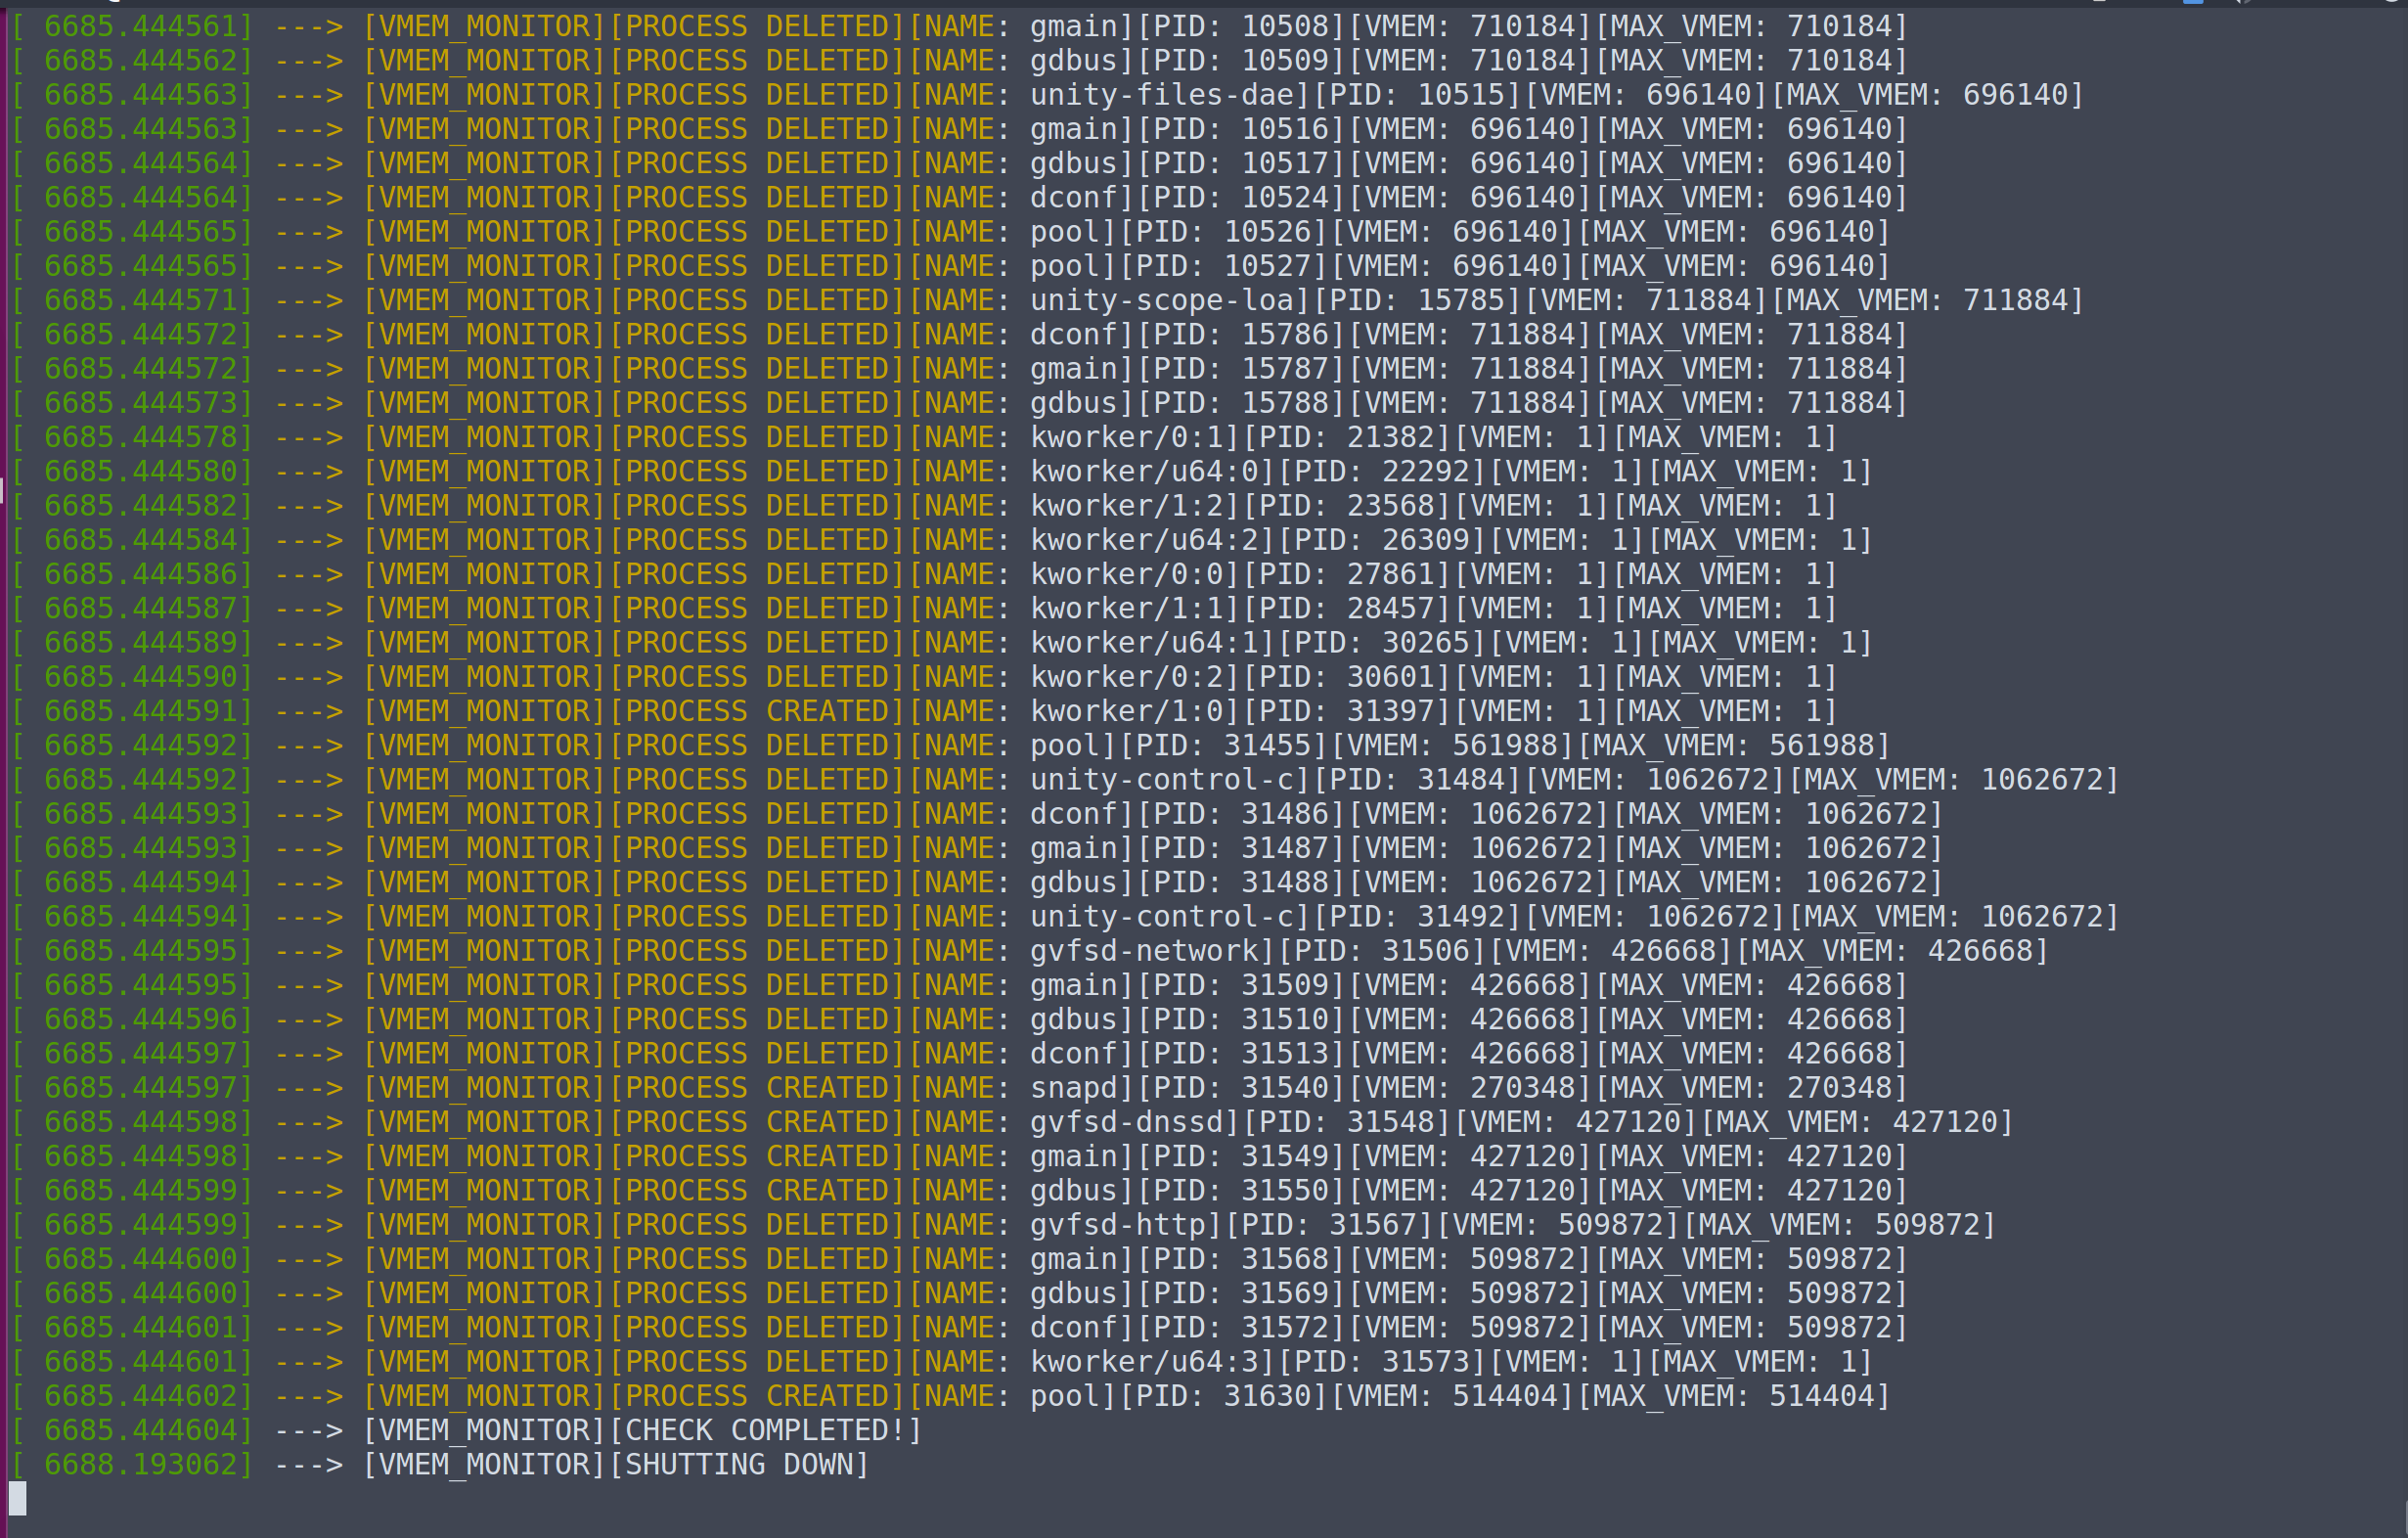
\includegraphics[width=\textwidth]{images/vmem_output}
 
 
 \subsection{پیاده سازی ماژول در سیستم‌عامل اندروید}
 برای ساخت ماژول در سیستم‌عامل اندرید، ابتدا فایل سورس کرنل مربوط به سیستم خودمان را از 
 \lr{kernel.org}
 دریافت می‌کنیم.
 سپس فایل Makefile را تغییر می‌دهیم تا به محل سورس کرنل اشاره کند:

\begin{latin}
\begin{verbatim}
obj-m += vmem.o

all:
    make -C /data/data/com.termux/files/home/linux-4.9.54 M=$(shell pwd) modules

clean:
    make -C /data/data/com.termux/files/home/linux-4.9.54 M=$(shell pwd) clean

\end{verbatim}	
\end{latin}

در نهایت ماژول را کامپایل می‌کنیم و آن را در هسته بارگزاری می‌نماییم.
\cite{8}
 
\begin{latin}
\begin{verbatim}
$ uname -r
> 4.9.54-android-x86_64-gfb63269e5ada
$ wget https://cdn.kernel.org/pub/linux/kernel/v4.x/linux-4.9.54.tar.xz
$ tar -xvf linux-4.9.54.tar.xz
$ vim Makefile
$ make
$ su
# insmod vmem.ko
\end{verbatim}	
\end{latin}

\section{گام سوم - پیاده سازی یک shell در سیستم عامل اندروید}
shell 
پیاده سازی شده توسط ما (\lr{DragonShell - dsh}) از shell ای که به عنوان پرسش آزمون پایانی درس ALP
\LTRfootnote{Advanced Linux Programming}
مطرح شده بود الهام گرفته شده است.

\subsection{آرگومان‌های ورودی}
این shell از آرگومان‌های زیر پشتیبانی می‌کند:
\begin{enumerate}
\item \lr{--logput <file>} یا \lr{-l <file>}
این آرگومان امکان تخصیص فایلی به عنوان log-file برای shell مهیا می‌کند. به این صورت که گزارشی از تمامی اتفاقات رخ داده در آن session در این فایل نوشته خواهد شد.

\item \lr{--user} یا \lr{-u}
این آرگومان نام کاربر فعلی سیستم را قبل از تمامی command های ورودی نمایش خواهد داد.

\item \lr{--hostname} یا \lr{-h}
این آرگومان نام session یا سیستم را قبل از تمامی command های ورودی و با علامت \@ نمایش خواهد داد.

\item \lr{--binpath <path(es)>} یا \lr{-b <path(es)>}
این آرگومان امکان ویرایش متغیر محیطی PATH را برای این session مهیا می‌کند. به گونه‌ای که از آدرس ارائه شده برای گشتن به دنبال فایل‌های binary دستورات استفاده خواهد شد.

\item \lr{--time <seconds>} یا \lr{-t <seconds>}

shell 
به صورت پیش فرض هر ۵ ثانیه یک بار تاریخ و ساعت فعلی را در فایل log ثبت می‌کند در صورتی که این آرگومان به برنامه داده شود می‌توان این دوره‌ی تناوب را بر حسب ثانیه تعیین کرد.
\end{enumerate}

برای parse  کردن این آرگومان‌ها از کتابخانه‌ی پیش‌فرض 
\lr{getopt.h}
استفاده شده است.

\subsection{توابع پیش‌فرض و داخلی}
برای پیاده سازی توابع پیش‌فرض و داخلی shell از ساختاری منعطف وگسترش پذیر استفاده کرده‌ایم. افزودن تابع جدید در آینده به این ساختار بسیار ساده  خواهد بود. برای این کار کافی است اشاره گر به تابع جدید را در لیست توابع پیش‌فرض اضافه کرده و نام آن را به لیست نام‌های توابع پیش‌فرض بیافزاییم و امضا و تعریف این تابع را نیز قید کنیم!

\begin{latin}
\begin{verbatim}
// builtin function signitures

int dsh_kill(char **args);
int dsh_cd(char **args);
int dsh_exit(char **args);
int dsh_help(char **args);

// builtin function name array

char *builtin_str[] = {
        "kill",
        "cd",
        "exit",
        "help",
};

// builtin function pointer arrays

int (*builtin_func[])(char **) = {
        &dsh_kill,
        &dsh_cd,
        &dsh_exit,
        &dsh_help,
};
int dsh_num_builtins() {return sizeof(builtin_str) / sizeof(char *);}

// builtin function implementations

int dsh_cd(char **args) {
    if (args[1] == NULL) {
        fprintf(stderr, "dsh: expected argument to \"cd\"\n");
    } else {
        if (chdir(args[1]) != 0) {
            perror("dsh");
        }
    }
    return 1;
}
int dsh_kill(char **args) {
    return 1;
}
int dsh_exit(char **args) {
    fprintf(stdout, "Good Luck!\n");
    return 0;
}
int dsh_help(char **args) {
    fprintf(stdout, "dragon shell v0.2!\n");
    fprintf(stdout, "By   Mohammadmahdi Faryabi!\n");
    fprintf(stdout, "   & Mohammadhosein A'lami!\n");
    return 1;
}
\end{verbatim}	
\end{latin}

یکی از مهمترین توابع پیش‌فرضی که پیاده سازی کرده‌ایم تابع  cd یا
\lr{change directory}
است. از آنجایی که directory فعال یکی از ویژگی‌های هر پردازه‌ است، فراخوانی این دستور بایستی منجر به یک syscall درون کد shell شود و نه اجرای یک فایل باینری دیگر. پس این دستور یک دستور داخلی shell است.

\subsection{مدیریت زمان و حافظه}
برای مدیریت حافظه از یک ریسه‌ی جداگانه استفاده کرده‌ایم. به این صورت مدیر حافظه وظیفه‌ی ثبت زمان در فایل log را بر عهده خواهد داشت.
 
سعی شده در مصرف حافظه‌ در dragon shell نهایت دقت به خرج داده شود. به این صورت حافظه‌ی مورد استفاده بلافاصله بعد از رفع نیاز به آن free می‌شود تا شاهد \lr{Memory Leakage} نباشیم.

\subsection{اجرا بر روی سیستم‌عامل لینوکس و اندروید}
تصاویر زیر مثال‌هایی از روال اجرایی shell روی سیستم‌های عامل لینوکس و اندروید را نمایش می‌دهند:

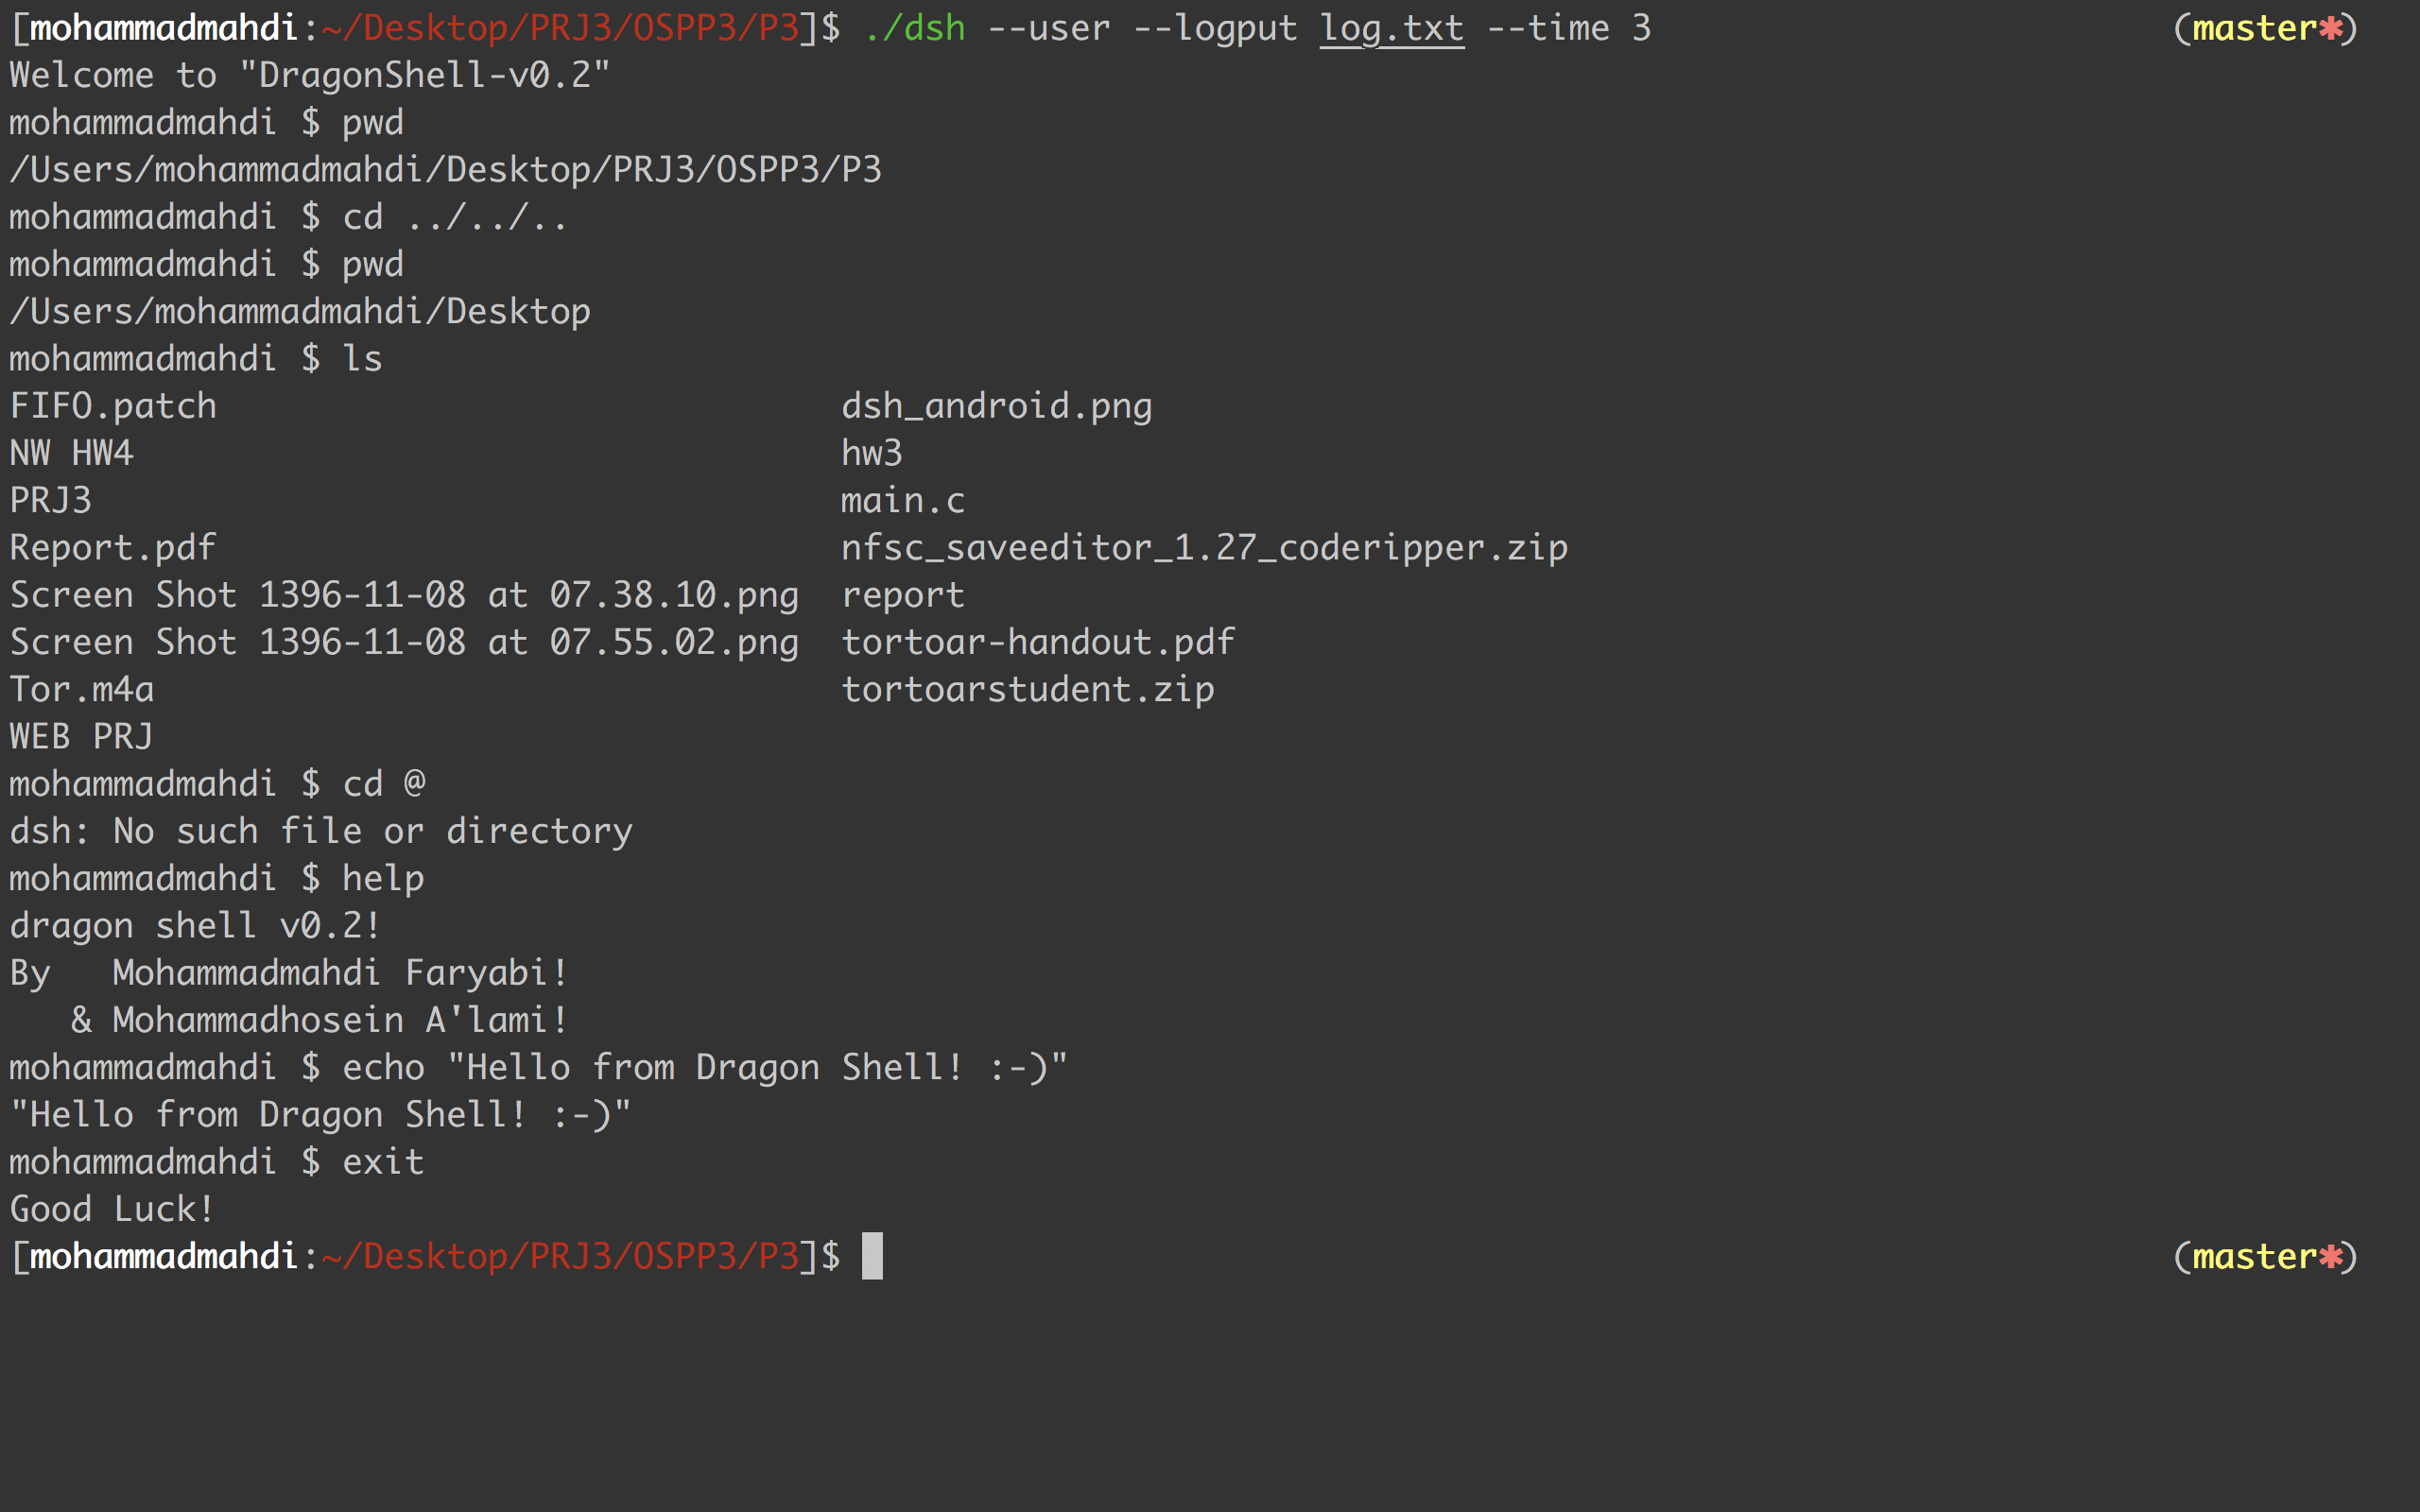
\includegraphics[width=\textwidth]{images/dsh_mac}
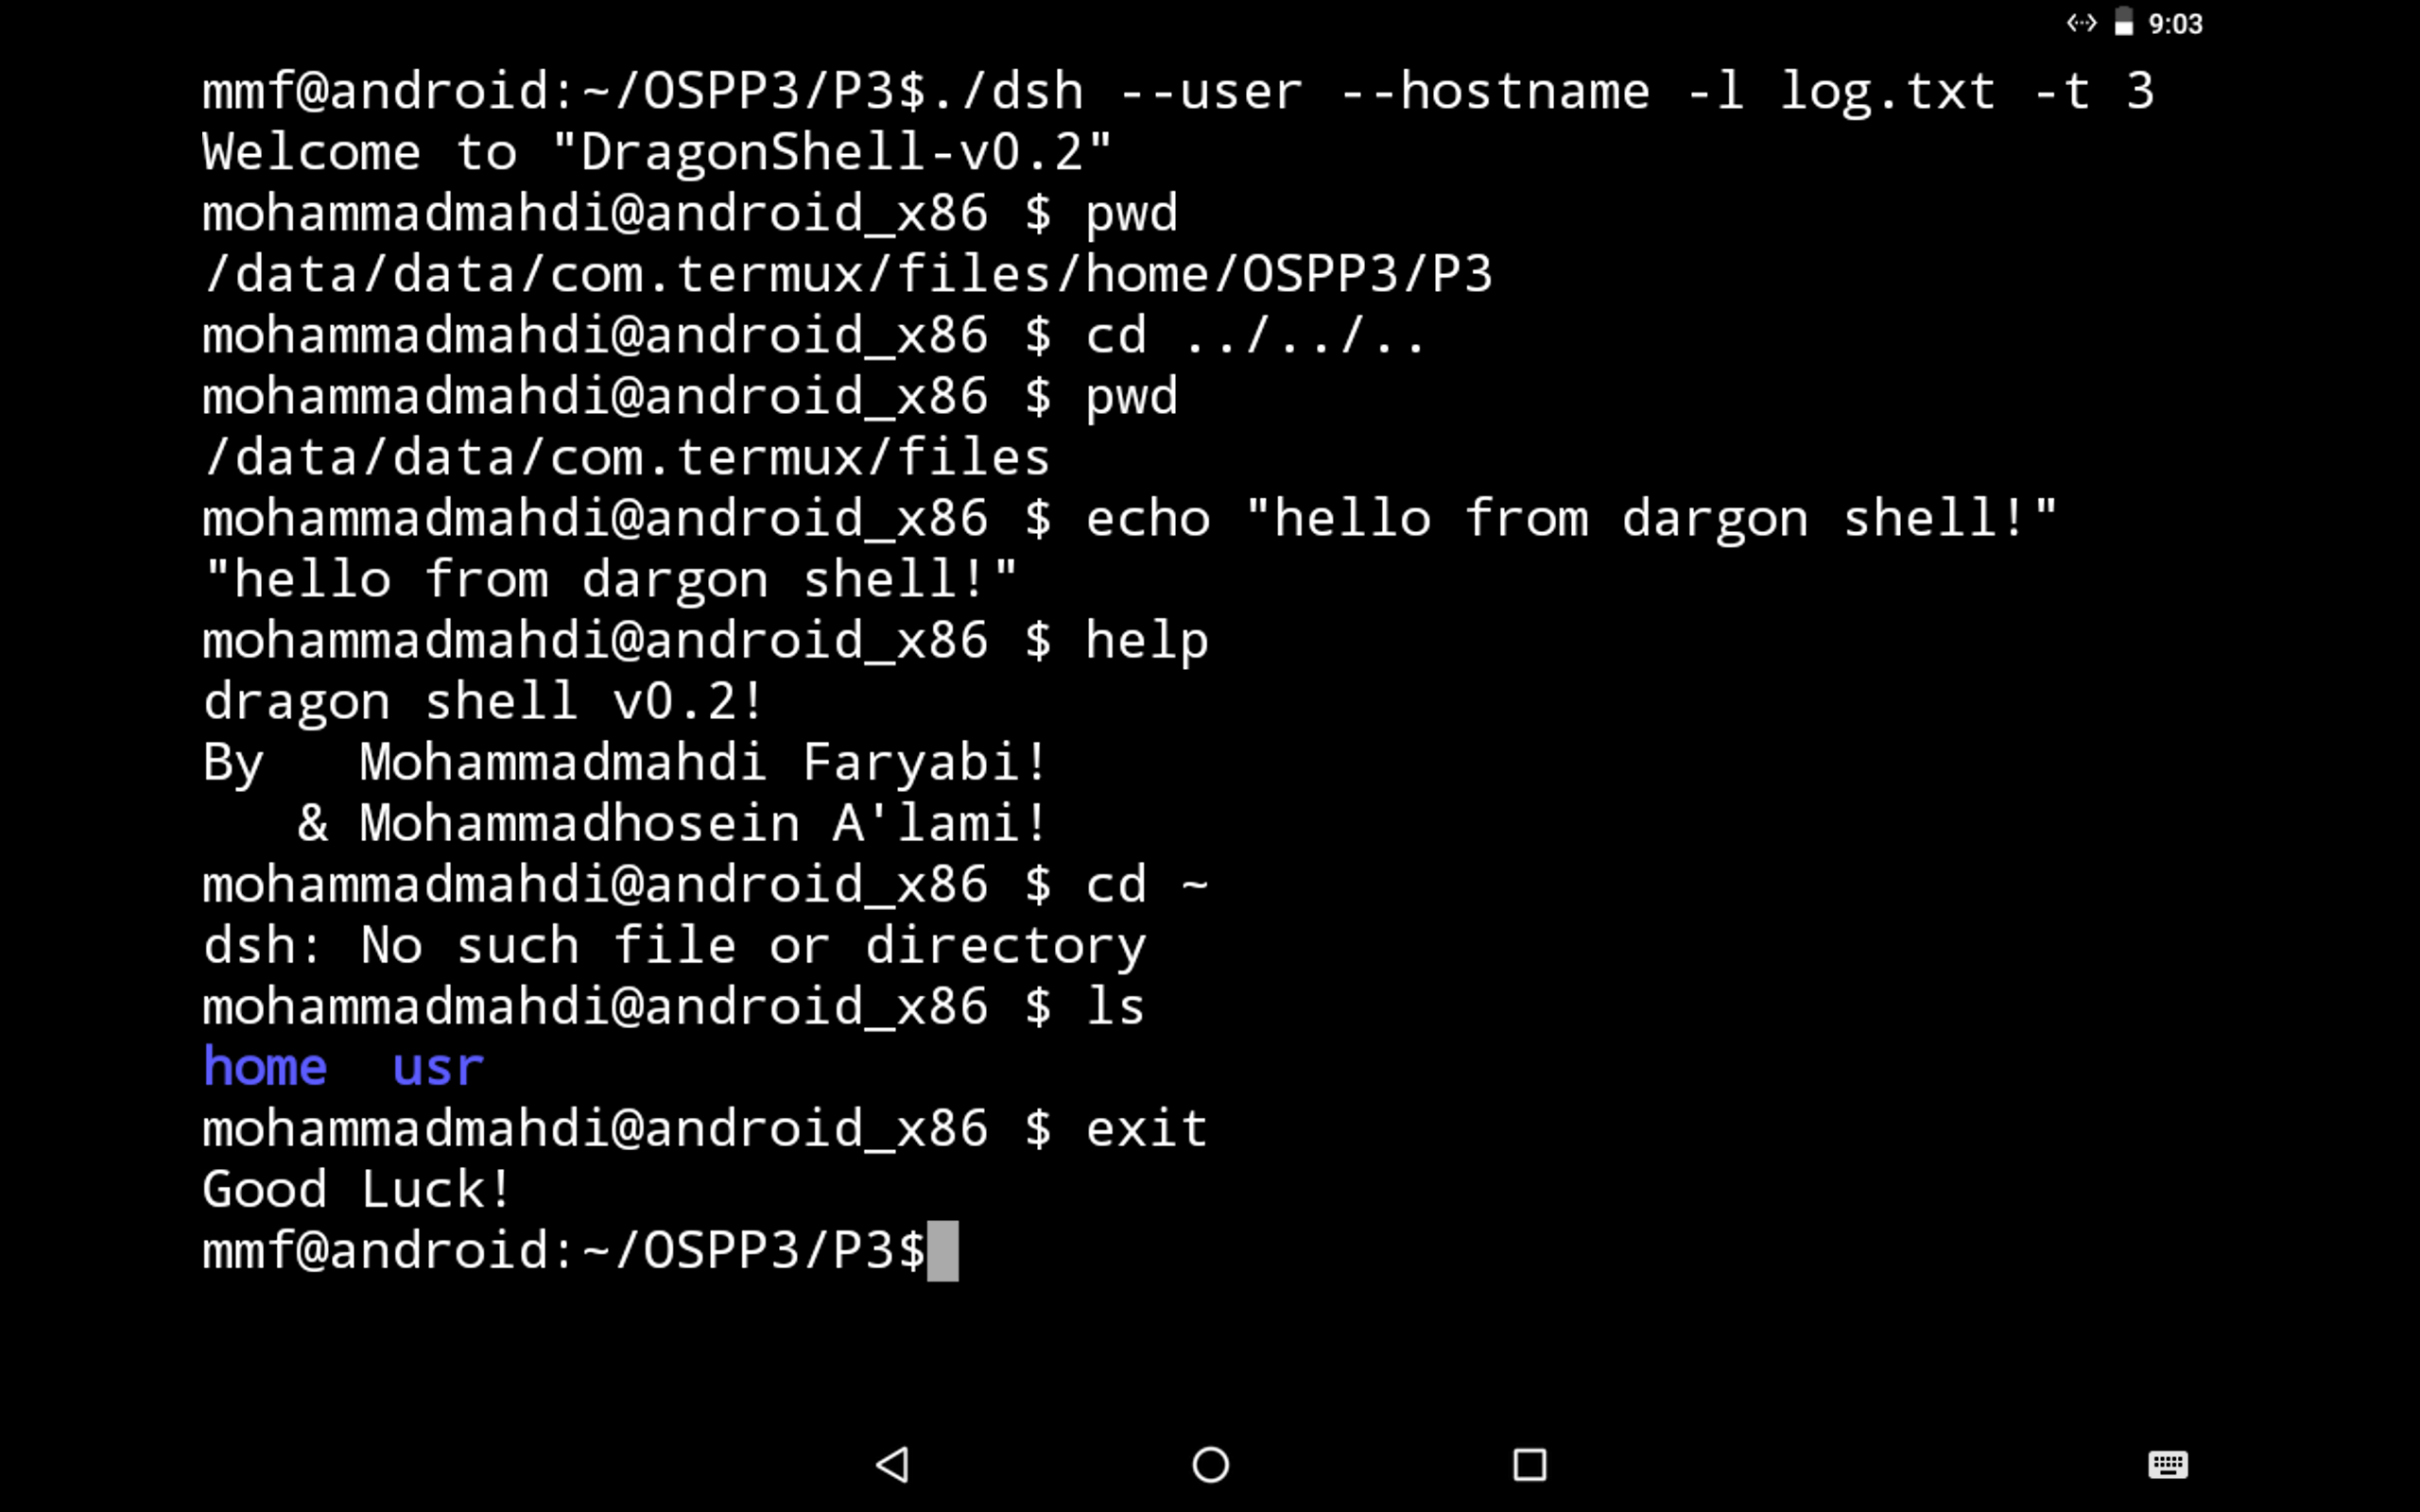
\includegraphics[width=\textwidth]{images/dsh_android}

در اینجا محتوای یک log-file نمونه را آورده‌ایم. مشاهده می‌شود که تمامی تعاملات کاربر با shell و خروجی دستورات log شده است:

\begin{latin}
\begin{verbatim}
CMD: pwd
RETVAL: 0
CMD: cd ../../..
CMD: pwd
RETVAL: 0
CMD: ls
RETVAL: 0
CMD: cd @
CMD: help
CMD: echo "Hello from Dragon Shell! :-)"
RETVAL: 0
CMD: exit
\end{verbatim}
\end{latin} 

\section{سیستم \lr{continuous Integration}، بورد trello و مخزن گیت}
تمامی فعالیت‌ها و کد‌های تولید شده روی مخزن گیت به آدرس 
\lr{\url{https://github.com/faryabimm/OSPP3}}
قرار دارد. همچنین هماهنگی‌ها و تقسیم‌کار از طریق بورد trello ی  پروژه به آدرس 
\lr{\url{https://trello.com/b/FSd9ukLa/os-course-project}}
انجام شده است.

در نهایت تمامی فرایند‌های ساخت توسط \lr{travis CI} و به صورت بر خط و مداوم انجام شده است.

\begin{thebibliography}{9}

\latin
\bibitem{1}
Robert Love. 2010. Linux Kernel Development (3rd ed.). Addison-Wesley Professional.
\bibitem{2}
A complete guide to Linux process schedulin, Nikita Ishkov
\bibitem{3}
\url{https://doc.opensuse.org/documentation/leap/tuning/html/book.sle.tuning/cha.tuning.taskscheduler.html}
\bibitem{4}
\url{https://www.systutorials.com/239998/sched_min_granularity_ns-sched_latency_ns-cfs-affect-timeslice-processes/?hilite=%27time%27%2C%27slice%27}
\bibitem{5}
\url{https://stackoverflow.com/questions/41957088/linux-default-scheduler-alternatives}
\bibitem{6}
\url{https://courses.linuxchix.org/kernel-hacking-2002/11-creating-applying-and-submitting-patches.html}
\bibitem{7}
\url{https://github.com/torvalds/linux}

\bibitem{8}
\url{https://rechtzeit.wordpress.com/2011/03/21/77/}

\bibitem{9}
\url{https://stackoverflow.com/questions/1184274/how-to-read-write-files-within-a-linux-kernel-module}

\bibitem{10}
\url{https://qnaplus.com/how-to-implement-periodic-timer-in-linux-kernel/}

\bibitem{11}
\url{https://brennan.io/2015/01/16/write-a-shell-in-c/}
\end{thebibliography}




\end{document}